% Created 2012-12-13 Thu 18:09
\documentclass[10pt, conference]{IEEEtran}
\usepackage[utf8]{inputenc}
\usepackage[T1]{fontenc}
\usepackage{fixltx2e}
\usepackage{graphicx}
\usepackage{longtable}
\usepackage{float}
\usepackage{wrapfig}
\usepackage{soul}
\usepackage{textcomp}
\usepackage{marvosym}
\usepackage{wasysym}
\usepackage{latexsym}
\usepackage{amssymb}
\usepackage{hyperref}
\tolerance=1000
\usepackage{balance}
\usepackage[numbers]{natbib}
\usepackage{graphicx}
\usepackage{dsfont}
\usepackage{mathtools}
\usepackage{amsmath}
\usepackage{subfigure}
\usepackage{multirow} %For tables
\usepackage{pdflscape}
\usepackage{rotating}
\usepackage{tabularx}
\usepackage{amsfonts}
\usepackage{booktabs}
\usepackage[amssymb]{SIunits}
\usepackage{fancyhdr}
\usepackage[format=hang,font=small,labelfont=bf]{caption}
\usepackage{hyperref}
\newcount\colveccount
\newcommand*\colvec[1]{\global\colveccount#1 \begin{bmatrix} \colvecnext }
\def\colvecnext#1{ #1 \global\advance\colveccount-1 \ifnum\colveccount>0 \expandafter\colvecnext \else \end{bmatrix}^{\top}\fi}
\providecommand{\alert}[1]{\textbf{#1}}

\title{Tool Use via Inverse Kinematics}
\author{Adam Cantor, Jonathan Martin, Leo Keselman, Stewart Butler}
\date{2012-12-10 Mon}
\hypersetup{
  pdfkeywords={},
  pdfsubject={},
  pdfcreator={Emacs Org-mode version 7.8.11}}

\begin{document}

\maketitle






\begin{abstract}
This report details an approach to known object interaction with a
Schunk Arm. A motion planning theorem is applied with a focus on
workspace control. The implementation of this system was done in the
GRIP/DART simulation environment designed/used by the Golems Lab at
Georgia Tech.
\end{abstract}

\section{Introduction}
\label{sec-1}

  The purpose of this work is to create a methodology for interacting
  with known objects in a loosely defined workspace. This goal is
  directly in line with the DARPA robotics challenge to apply humanoid
  robots to search and rescue applications by using tools and
  exploration algorithms.

  No single robot can be equipped to deal with all environments equally
  well. A general purpose robot, given a concrete goal for which it is
  not configured correctly, must be able to use objects from its
  environment to reach its goals. In an anthropocentric environment this
  means that correctly wielding tools designed for human use gives a
  robot a degree of operational flexibility that would be otherwise
  impossible.


\begin{figure}[htb]
\centering
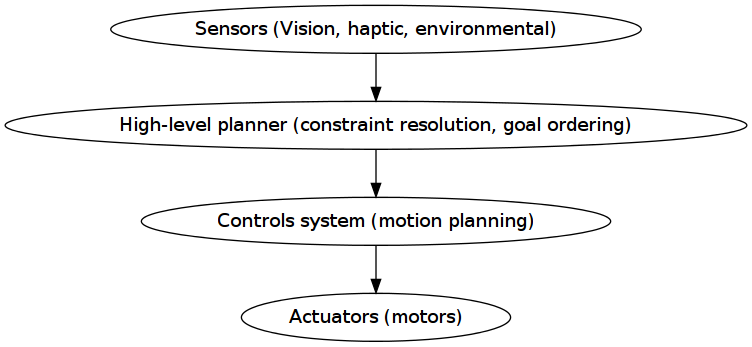
\includegraphics[width=8cm]{robot_layer_model_04acea6317138ac7fb5e808de063a70455ba7e53.png}
\caption{\label{fig:layer_model}Layer model of robot control systems.}
\end{figure}


  Using human-configured tools requires multiple layers of control and
  planning, as shown in figure \ref{fig:layer_model}.

\begin{enumerate}
\item Sensors - The robot must be capable of discerning its environment,
     discovering what constraints that environment will impose upon it,
     and constructing sub-goals in order to accomplish its target
     task. In an un-augmented anthropocentric environment, this means
     having a sufficiently sophisticated computer vision system (visual,
     radar, lidar, etc) to map the environment, recognize objects in the
     environment, and classify them as a given tool. It also means using
     haptic feedback (if possible) and torque feedback from the
     actuators during manipulation tasks as part of a control loop to
     ensure that the manipulated objects are behaving according to
     plan.
\item Planner - The robot needs a high level planner in order to take a
     goal state, break it into sub goals, match those sub goals with
     tasks it is able to handle, resolve any dependency conflicts, and
     order those goals into as efficient a plan as possible.
\item The control system is responsible for implementing each of the
     tasks necessary to accomplish a given sub-goal. This involves
     things like the lower-level motion planning necessary for
     manipulation, including workspace control.
\item Actuators - The robot must be capable of using its actuators to
     accomplish commands sent to them from the control
     system. Physically, one must be able to manipulate the tool in
     question. General purpose manipulators are not generally well
     suited for using tools designed for humanoid hands, and most
     commonly available humanoid hands have issues with grip strength,
     digit control, haptic sensing, and friction.
\end{enumerate}

  This document describes an effort to explore the challenges associated
  with general purpose tool usage from within a simulated
  environment. To reduce the scope of an otherwise unmanageable problem,
  the goal was simplified to be the control system for a single
  simulated Schunk LWA-4 arm, a 7-degree-of-freedom arm with an
  attachable manipulator. A screwdriver was chosen as the target tool,
  since it is the simplest tool that could be easily manipulated by a
  Schunk arm and still require a complex set of actions. In order to
  remove the necessity for a complicated sensor system, the work was
  done using the GRIP/DART simulation environment used by the Humanoid
  Robotics laboratory at Georgia Tech.

  Complications arose during the work which prevented all our goals from
  being reached. The implementation of the vital control elements of the
  proposed system was unusable due to bugs in the implemented workspace
  control. These were fixed to a usable point, but there was not enough
  time remaining to integrate the high level planner into the decision
  loop. As such, the robot is capable of all the physical manipulation
  tasks needed to reach its goal state, but those states must be
  manually traversed by a human in order for the simulation to
  work. These issues will be further discussed in later sections.
\section{Related Work}
\label{sec-2}

  Tool manipulation in workspace is very common in both research and
  industry. However, most of this tool manipulation is with specialized
  tools that are not designed for human manipulation, and the robots are
  generally used in environments where the state space is largely
  deterministic -- the planner for the robot can safely assume that a
  part will enter the assembly line at a certain time, reach a certain
  location in a certain orientation, and if there are any deviations
  from this expected behavior it will simply stop and alert a human of a
  problem.

  What made our planned approach unique is that we account both for the
  motion planning for the robot as well as the constraints of the
  tool. For example, when driving the screw into the target block, we
  must follow the screw with the driver (held in the manipulator) as it
  threads into the target block by matching `downward' translation with
  the rotation of the screw driver, then back the tool out and repeat
  until the screw is settled into the block. It also took into account
  the set of actions required to set up the environment -- finding the
  screw, placing it in the correct location for tool use, finding the
  tool, and finally driving the screw into the target block.

  [Tucker]
  [general grasp]
\section{Methods}
\label{sec-3}
\subsection{Simulation Software}
\label{sec-3-1}


  In the current experiments, there are three interactive objects and
  one robot arm. The interactive objects are a screwdriver, a bolt, and
  a goal block, all located within the arm's range of movement.

  Our system then follows the following set of actions to generate a
  plan.
\subsection{High Level Planning}
\label{sec-3-2}
\subsubsection{Locate screw}
\label{sec-3-2-1}

    After the screw is inserted into the world file, it is passed to the
    robot as a motion goal point. The robot queries the world to find the
    object and obtains the transform of the current tool position in the
    world's coordinate reference frame. The 4x4 affine matrix
    representing the rotation and translation of the screw is then
    converted into a 6x1 vector:
    \begin{equation}
    q = \begin{bmatrix}
                a \\
                w
              \end{bmatrix}
    \end{equation}

    Here, \(a\) is a three dimensional translation vector and \(w\)
    is a roll, pitch, and yaw vector relative the world origin which
    define the origin of the screw.
\subsubsection{Grasp the screw}
\label{sec-3-2-2}

    Jacobian workspace control is used to align the robot's manipulator
    with the coordinate frame of the screw. After matching rotation and
    position with the target, the robot grabs the screw. Subsequently,
    the screw is manipulated as though it were an additional link in the
    arm.
\subsubsection{Locate goal}
\label{sec-3-2-3}

\begin{enumerate}
\item Move the bolt to alignment with the goal.
\end{enumerate}
\subsubsection{Release bolt}
\label{sec-3-2-4}
\subsubsection{Grasping tool}
\label{sec-3-2-5}

    Grasp the screwdriver; updating the end effector after each
      interaction.
\subsubsection{Move tool to screw}
\label{sec-3-2-6}

    After moving the screwdriver into the bolt, update the arm to include
      the bolt as well
\subsubsection{Drive screw into goal point}
\label{sec-3-2-7}

    Moving it into the goal position.
\subsubsection{Release bolt}
\label{sec-3-2-8}

   Release the bolt
\subsubsection{Release tool}
\label{sec-3-2-9}

    Replace the screwdriver back to its original position.
\subsection{Low Level (Motion) Planning}
\label{sec-3-3}
\subsubsection{Resolved Rate Trajectory Planning}
\label{sec-3-3-1}

    Resolved rate trajectory planning, or pseudo-inverse Jacobian
    control, was used to move the manipulator from a current world
    configuration \( \mathbf{x_i} =
    \colvec{6}{x_i}{y_i}{z_i}{R_i}{P_i}{Y_i} \) to a target goal
    configuratfon \( \mathbf{x_f} =
    \colvec{6}{x_f}{y_f}{z_f}{R_f}{P_f}{Y_f}\) in a linear fashion. The
    world coordinates are described as \( 6 \times 1 \) vectors of X,Y,
    and Z positions with corresponding Roll, Pitch and Yaw.

    Resolved rate trajectory control stems from
    \ref{ eq:rate_trajectory}, where \(\mathbf{V_e}(t)\) is the end
    effector velocity at time \(t\), \(\mathbf{\alpha}\) is the joint
    space position vector describing the current configuration of the
    robot, and \(\textbf{\dot{\alpha}}\) is the joint space velocity
    vector.

    \begin{equation}
    \label{ eq:rate_trajectory}
    \mathbf{V_{e}}(t)\mathbf{ = J(\alpha)\dot{\alpha}}
    \end{equation}

    This can be rearranged into \ref{eq:rate_trajectory_inv}.

    \begin{equation}
    \label{eq:rate_trajectory_inv}
    \mathbf{\dot{\alpha} = J^{-1}V_e(t)}.
    \end{equation}

    Thus, if the inverse Jacobian and desired end effector trajectory
    are known, it is possible to make a differential equation for the
    joint angles of the manipulator. In this case, the trajectory is to
    be linear, so \(\mathbf{V_e(t)}\) was a constant \(6 \times 1\) vector equal
    to \(\mathbf{x_f}-\mathbf{x_i}\).
\begin{itemize}

\item Extracting a target coordinate\\
\label{sec-3-3-1-1}%
The world coordinate of a given node is generated from DART/GRIP as
     an affine transformation described by the \(4 \times 4\)
     homogeneous coordinate matrix \(C = \begin{bmatrix}
     \multicolumn{3}{c}{\mathbf{R}} & \mathbf{X_{xyz}} \\ 0 & 0 & 0 & 1 \end{bmatrix}\),
     so the \(6 \times 1\) XYZRPY vector representation must first be
     extracted.

     \(\mathbf{X_{xyz}}\) is a \(3 \times 1\) vector describing a point in
     3-space, and does not require any manipulation. \(\mathbf{R}\) is a \(3
     \times 3\) rotation matrix, so we convert this to roll-pitch-yaw as
     shown in equation \ref{eq:rpy}:

     \begin{equation}
     \label{eq:rpy}
     \mathbf{X_{rpy}} = \begin{bmatrix} \tan^{-1}(\frac{R_{2,1}}{R_{2,2}}) \\
     -\sin^{-1}(R_{2,0}) \\ \tan^{-1}(\frac{R_{1,0}}{R_{0,0}}) \end{bmatrix},
     \end{equation}

     This yields our target coordinates \(\mathbf{x_{f}}
     = \begin{bmatrix}X_{xyz} \\ X_{rpy} \end{bmatrix} \).


\item Inverting the Jacobian\\
\label{sec-3-3-1-2}%
A direct inverse of the Jacobian is not possible in our case, as
     our manipulator had 7 degrees of freedom producing a \(7 \times 6\)
     matrix. Instead, a Moore-Penrose pseudo-inverse was calculated
     according to equation \ref{eq:pseudoinv}.

     \begin{equation}
     \label{eq:pseudoinv}
     J^{\dagger} = J^{\top}(JJ^{\top})^{-1}
     \end{equation}

     From this we compute for each time step the change in joint angles
     via equation \ref{eq:velocity}:

     \begin{equation}
     \label{eq:velocity}
     \dot{\alpha} = J(\alpha)^{\dagger}V_e(t)
     \end{equation}

     This is added to the previous time step's joint configuration and
     the robot is updated. The process continues until the global
     coordinates (both rotation and translation) of the end effector
     of the manipulator is less than a threshold distance $\epsilon$
     of the desired position. In other words,

     \begin{equation}
     \label{eq:distance}
     \| \mathbf{x_f - x_i} \| < \epsilon
     \end{equation}


\item Joint limits\\
\label{sec-3-3-1-3}%
This equation for the joint velocities is not always well
     behaved. In order to improve the results, we will use a variation
     of the joint-limits avoidance strategy described in
     \cite{luc_baron}.

     We now know from \ref{eq:velocity} the regular form of our
     velocity equation used to generate a trajectory toward our primary
     task. We will now augment that with an additional secondary task
     that will bias the trajectory towards keeping the joints as close
     to their zero points as possible.

     First, we augment equation \ref{eq:velocity}, so our equation
     describing the change in joint angles is now \ref{eq:vel_jl}.

     \begin{equation}
     \label{eq:vel_jl}
     \mathbf{\dot{\alpha} = J_{\alpha}^{\dagger}V_e(t) + (1 -
     J_{\alpha}^{\dagger}J_{\alpha})h}
     \end{equation}

     The vector \(h\) is our secondary task, multiplied by \(\mathbf{
     (1 - J_{\alpha}^{\dagger}J_{\alpha})}\), the orthogonal complement
     of J$_{\alpha}$. The result is a projection of \(\mathbf{h}\) into
     the null space of \(\mathbf{J_\alpha}\), a ``virtual motion'' which
     results in a bias toward the secondary objective.

     The secondary task is constructed as  \(\mathbf{h} = \gradient z\),
     where \(z\) is a fitness function described in \ref{eq:z}.

     \begin{equation}
     \label{eq:z}
     \mathbf{ z = \frac{1}{2}(\alpha - \bar{\alpha})^{\top}W(\alpha -
     \bar{\alpha})}
     \end{equation}

     The variable \(\mathbf{\bar{\alpha}}\) is the joint position vector
     describing the mid-joint position; in our case, this is an all-zero
     vector, as the entire arm is constructed from symmetrically
     revolute joints centered around zero.

     The matrix \( \mathbf{W} \) is a diagonal weight matrix describing
     the acceptable deviation from this zero point -- if it is desirable
     for a particular joint to have a greater latitude during movement
     than another, altering the corresponding row in the weight matrix
     will generate that effect. In our case, an identity matrix was
     used, as we only needed a general bias away from the joint limits.

     The effect is that \(\mathbf{h}\) describes a gradient where the
     zero positions on each joint is a minima, growing steeper as you
     progress further away from this center point. When projected into
     the null space of \(\mathbf{J_\alpha}\), it will cause joints that
     are otherwise unconstrained by the target motion to descend toward
     their zero positions, preventing the robot from approaching too
     close to the joint limits and preventing some of the anomalous
     behavior produced by unconstrained inverse Jacobian control.

\end{itemize} % ends low level
\subsection{Object manipulation}
\label{sec-3-4}
\section{Experiments}
\label{sec-4}
\section{Analysis}
\label{sec-5}
\section{Discussion}
\label{sec-6}

\end{document}
